\documentclass[../main.tex]{subfiles}

\begin{document}

\chapter{Alogrithms}

This appendix details the applied encryption and decryption algorithms.

\section{Encryption algorithm}
\label{app:encryption}
\begin{figure}[h]
    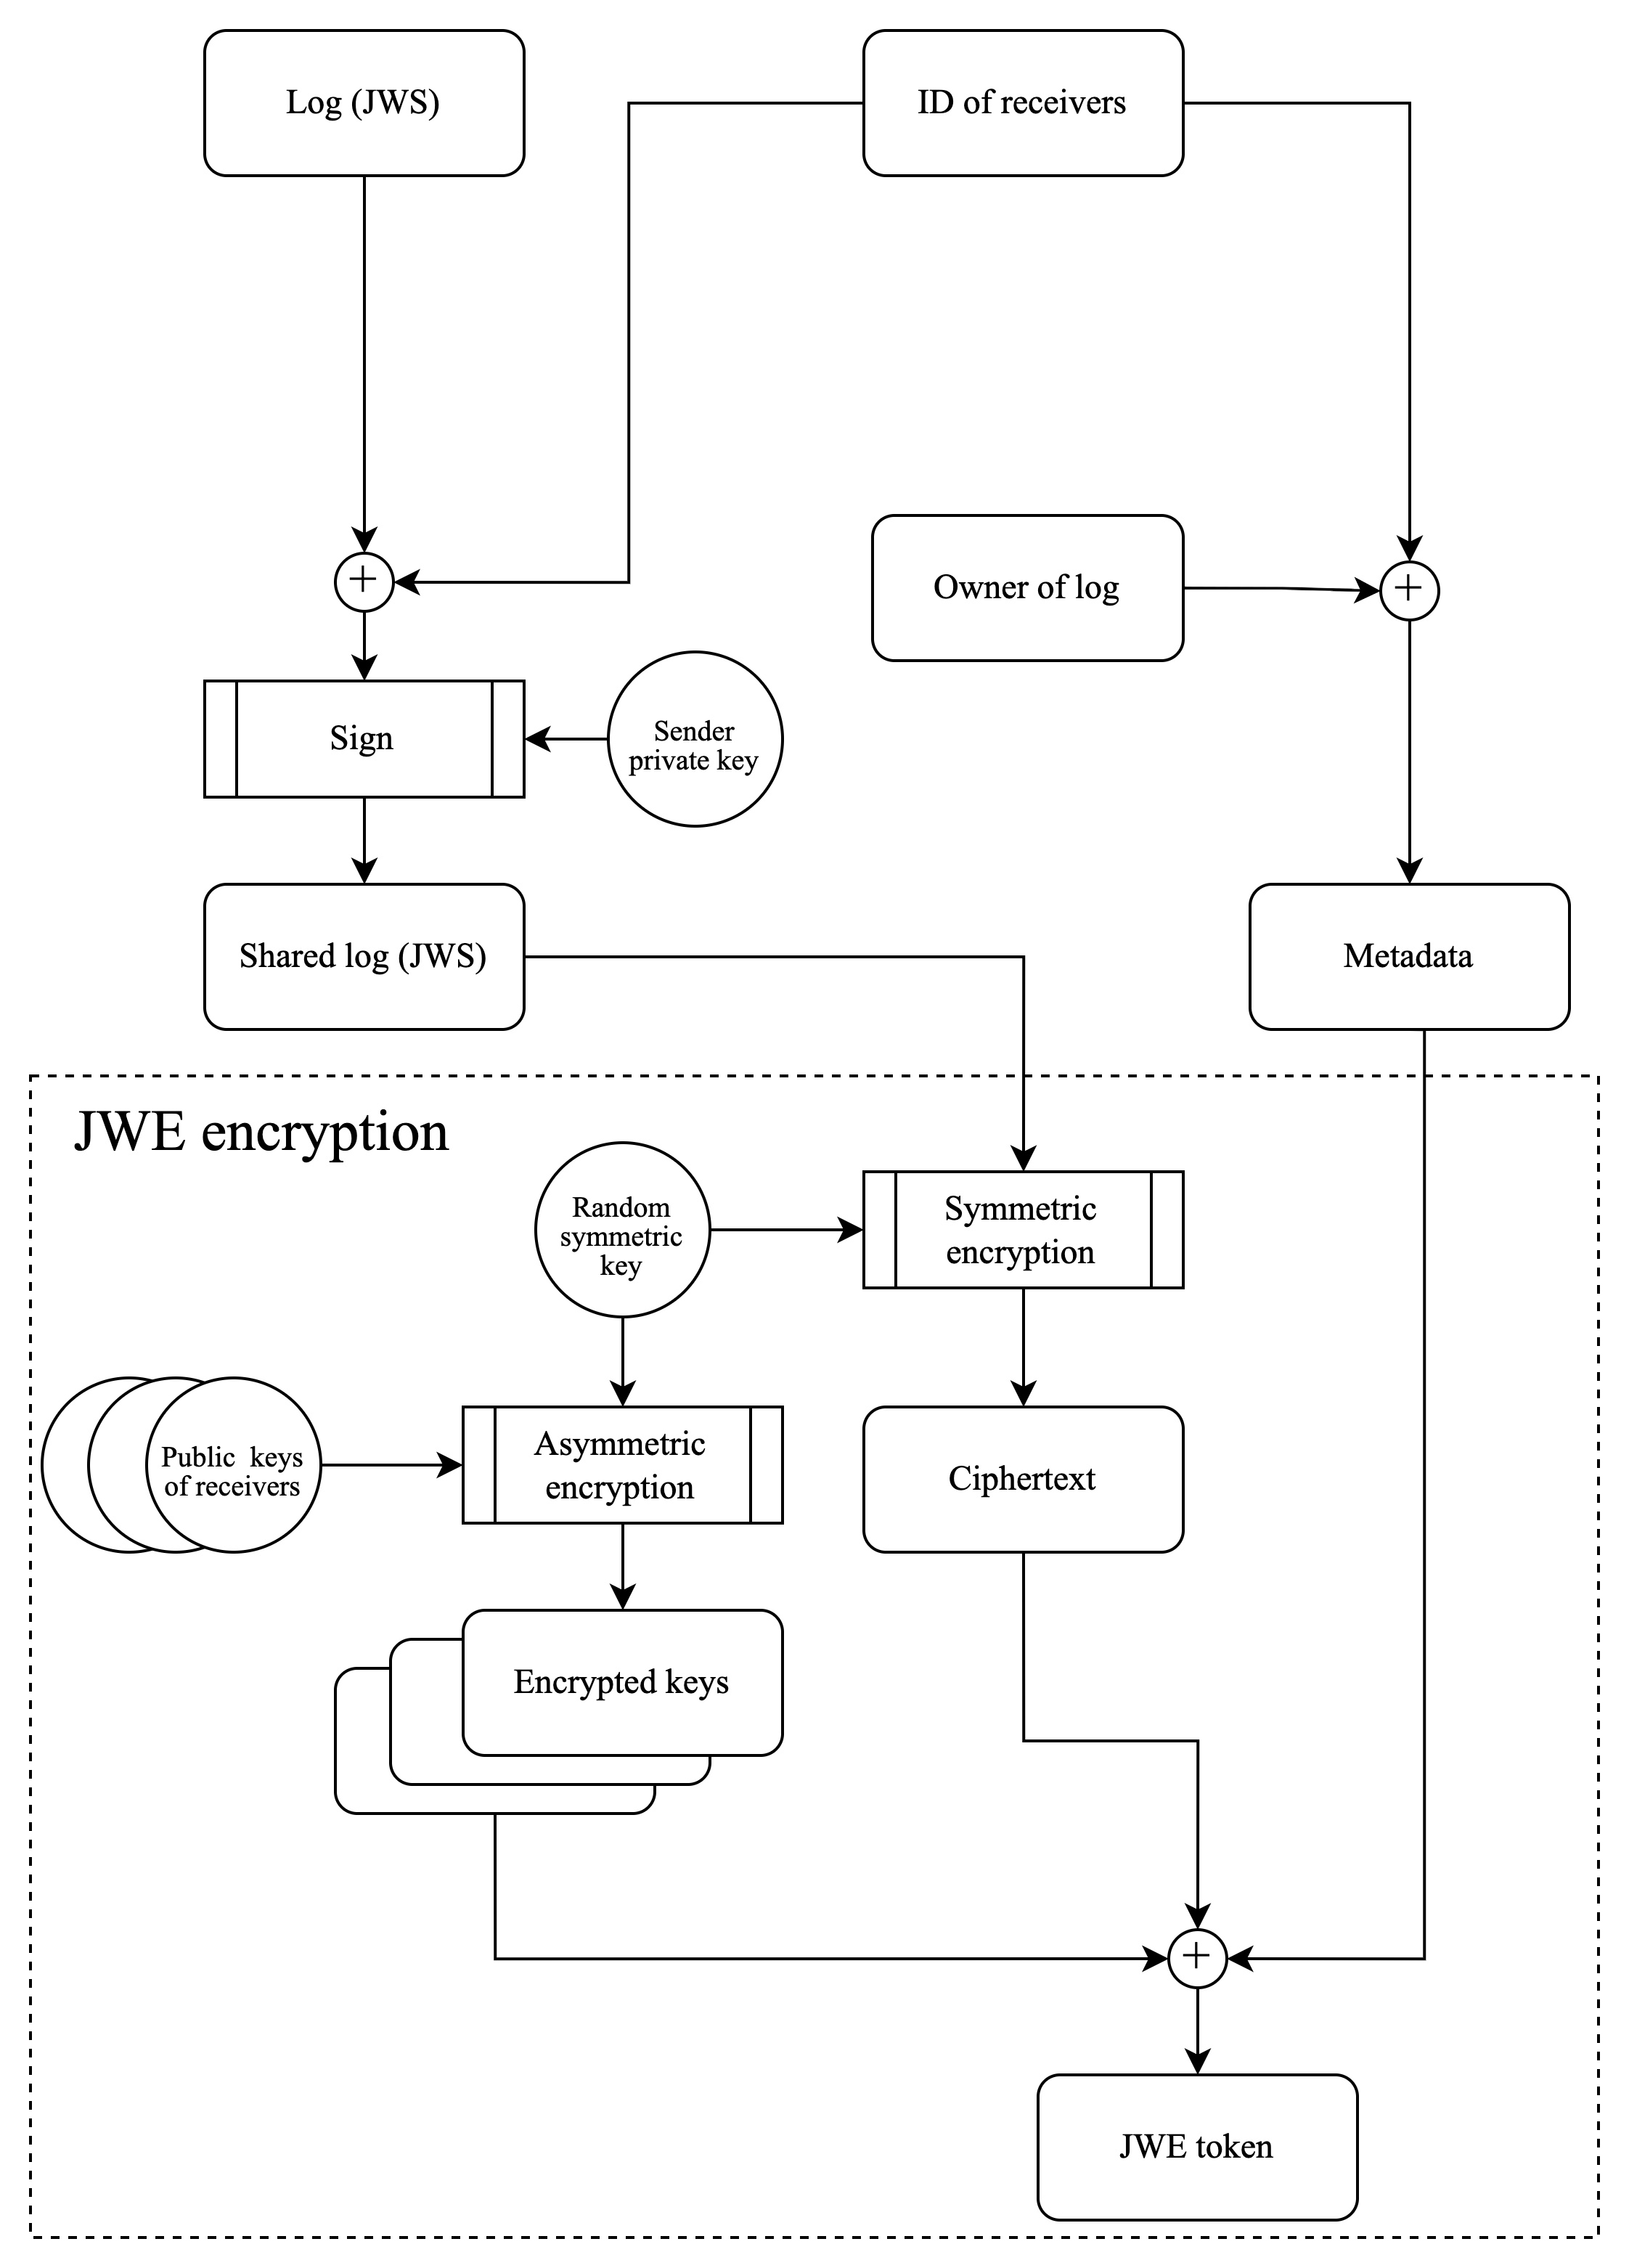
\includegraphics[scale=0.13]{../img/05/encrypt_logs.jpg}
    \centering
    \caption{The encryption algorithm takes a signed log and a set of receivers as input. It returns a JWE-token which can only be decrypted by the specified set of users.}
    \label{app:encryption_algo}
\end{figure}
\newpage
\section{Decryption algorithm}
\label{app:decryption}
\begin{figure}[h]
    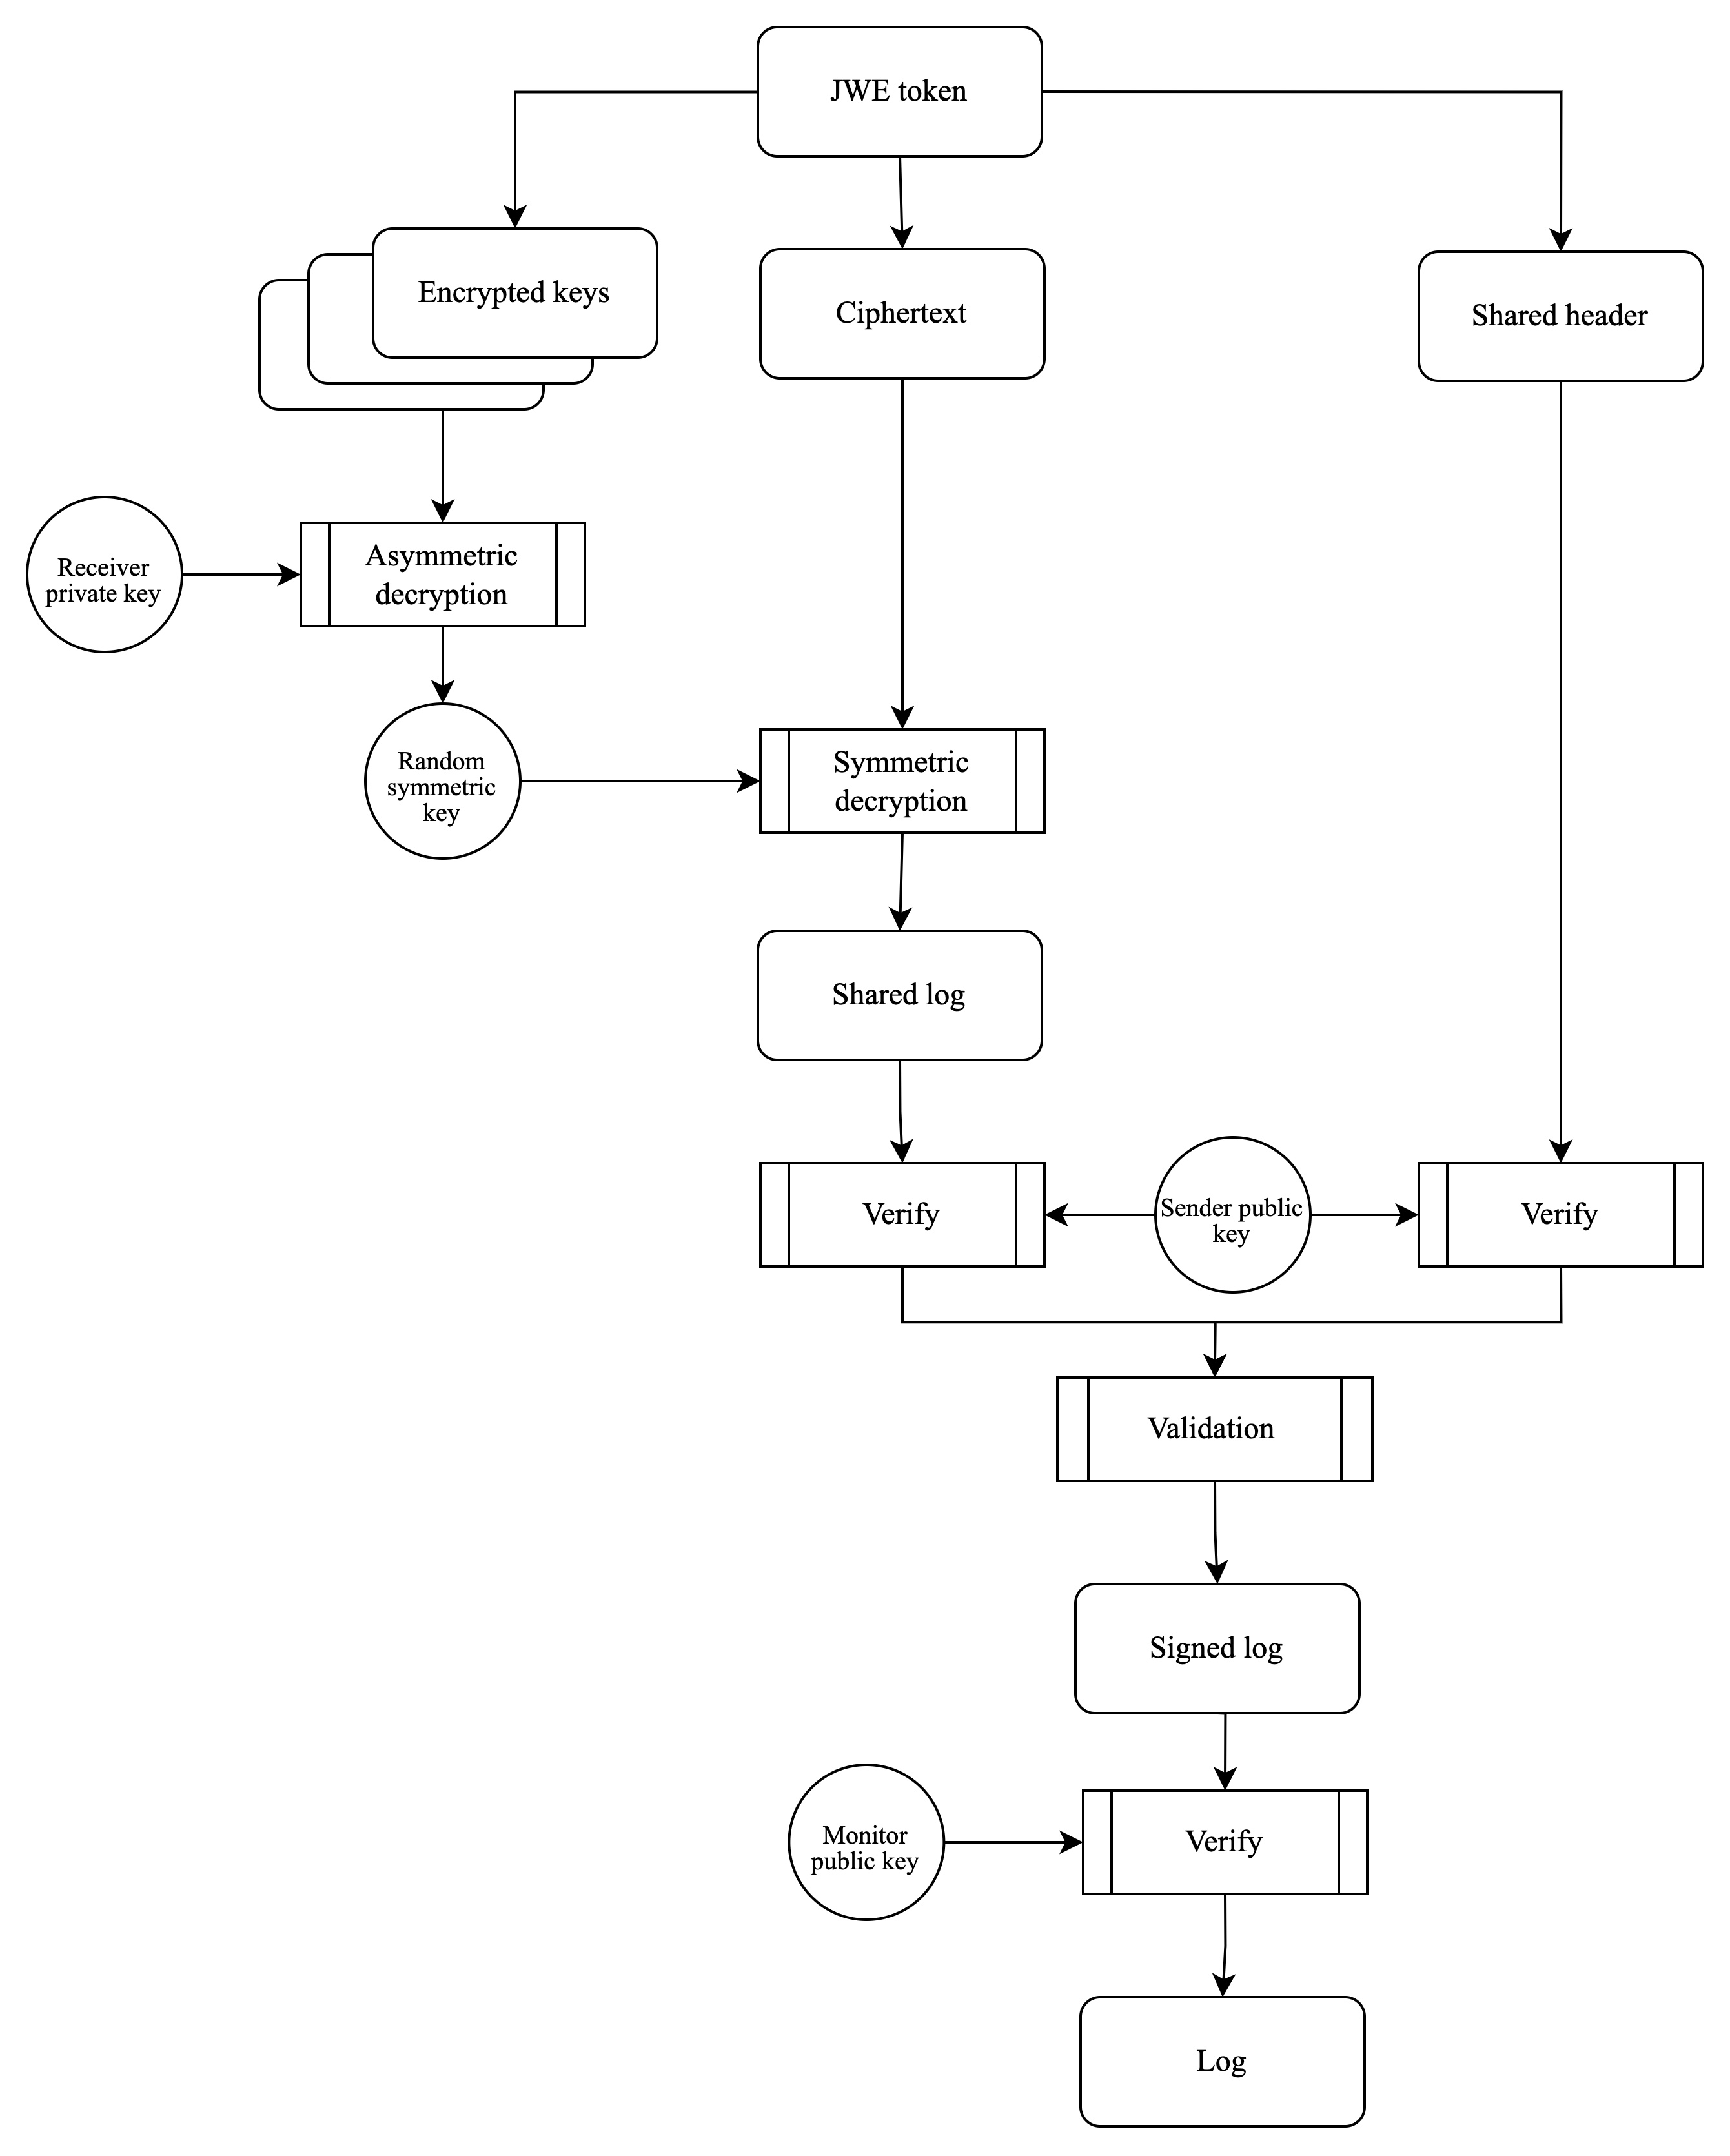
\includegraphics[scale=0.13]{../img/05/decrypt_logs.jpg}
    \centering
    \caption{The decryption algorithm takes a JWE token and a private decryption key as input. It returns the decrypted log if the user is allowed to decrypt.}
    \label{app:decryption_algo}
\end{figure}


\end{document}
